% \chapter{Vision}
\chapter{视觉}
\label{chap:vision}

% Vision is one of the information-rich sensor system both humans and robots have available. Processing the wealth of information that is generated by vision sensors is still a key challenge, however. The goal of this chapter is to introduce

视觉是人类和机器人可用的信息丰富的传感器系统之一。然而,处理由视觉传感器产生的丰富信息仍然是一个关键的挑战。本章的目的是介绍

\begin{itemize}
% \item images as two-dimensional signals,
% \item providing an intuition of the wealth of information hidden in low-level information,
% \item introducing basic convolution and threshold-based image processing algorithms.

\item 图像作为二维信号,
\item 提供隐藏在低级信息中的信息丰富的直觉,
\item 介绍基本卷积和基于阈值的图像处理算法。
\end{itemize}

% \section{Images as two-dimensional signals}
\section{图像作为二维信号}

% Images are captured by cameras containing matrices of charge-coupled devices (CCD) or similar semi-conductors that can turn photons into electrical signals. These matrices can be read out pixel by pixel and turned into digital values, for example an array of 640 by 480 three-byte tuples corresponding to the red, green, and blue (RGB) components the camera has seen. An example of such data, for simplicity only one color channel, is shown in Figure \ref{fig:iss_closeup}. 

% Looking at the data clearly reveals the white tile within the black tiles at the lower-right corner of the chessboard. Higher values correspond to brighter colors (white) and lower values to darker colors. We also observe that although the tiles have to have the same color, the actual values differ quite a bit. It might make sense to think about these values much like we would do if the data would be 1D signal: taking the ``derivative'', e.g., along the horizontal rows, would indicate areas of big changes, whereas the ``frequency'' of an image  would indicate how quickly values change. Areas with smooth gradients, e.g., black and white tiles, would then have low frequencies, whereas areas with strong gradients, would contain high frequency information. 

图像由包含可以将光子转换为电信号的电荷耦合器件(CCD)或类似半导体矩阵的相机捕获。这些矩阵可以逐个像素地读出并转换为数字值,例如相机所看到的与红色,绿色和蓝色(RGB)分量相对应的640×480三字节元组的数组。这种数据的一个例子,为简单起见,只有一个颜色通道,如图\ref{fig:iss_closeup}所示。

查看数据清楚地显示了棋盘右下角的黑色瓦片中的白色瓦片。较高的值对应于较亮的颜色(白色),较低的值对应于较暗的颜色。我们还观察到,尽管瓷砖必须具有相同的颜色,但实际值差异很大。如果数据是1D信号,那么考虑这些值就可能是有意义的:采取“衍生”,例如沿着水平行,将指示大变化的区域,而“频率”“一个图像将表明价值变化的速度。具有平滑梯度的区域(例如黑色和白色瓷砖)将具有低频率,而具有强梯度的区域将包含高频率信息。


\begin{figure}[!htb]
	\centering
		\includegraphics[width=\textwidth]{figs/iss_closeupmatrix}
	% \caption{A chessboard floating inside the ISS, astronaut Gregory Chamitoff. The inset shows a sample of the actual data recorded by the image sensor. One can clearly recognize the contours of the white tile.}
	\caption{漂浮在国际空间站内的棋盘,宇航员格雷格·坎日夫(Greg Chamitoff)。 插图显示了图像传感器记录的实际数据的样本。 可以清楚地识别白色瓷砖的轮廓。}
	\label{fig:iss_closeup}
\end{figure}

% This language opens the door to a series of signal processing concepts, such as low-pass filters (supressing high frequency information), high-pass filters (suppressing low frequency information), or band-pass filters (letting only a range of frequencies pass), analysis of the frequency spectrum of the image (the distribution of content at different frequencies), or ``convolving'' the image with another two-dimensional function. The next sections will provide both an intuition of what kind of meaningful information is hidden in such abstract data and provide concrete examples of signal processing techniques that make this information appear.

这种语言打开了一系列信号处理概念,例如低通滤波器(抑制高频信息),高通滤波器(抑制低频信息)或带通滤波器(仅允许频率范围通过)),分析图像的频谱(不同频率的内容分布),或者使用另一个二维函数“卷积”图像。下一节将提供在这些抽象数据中隐藏什么样的有意义的信息的直觉,并提供使信息出现的信号处理技术的具体示例。

% \section{From signals to information}
% Unfortunately, many phenomena that often have very different or even opposite meaning look very similar when looking at the low-level signal. For example, drastic changes in color values do not necessarily mean that the color of a surface indeed has changed. Similar patterns are generated by depth discontinuities, specular highlights, changing lighting conditions, or surface orientation changes. These examples are illustrated in Figure \ref{fig:iss_edges} and make computer vision a hard problem.  

\section{从信号到信息}
不幸的是,在观察低级信号时,许多通常具有非常不同或相反意义的现象看起来非常相似。例如,颜色值的剧烈变化不一定意味着表面的颜色确实已经改变。类似的图案由深度不连续性,镜面高光,改变照明条件或表面取向变化产生。这些例子如图\ref{fig:iss_edges}所示,使计算机视觉成为一个难题。


\begin{figure}[!htb]
	\centering
		\includegraphics[width=\textwidth]{figs/iss_edges}
	% \caption{Inside of the international space station (left), highlighted areas in which pixel values change drastically (right). Underlying effects that produce similar responses: change in surface properties (1), depth discontinuities (2), specular highlights (3), changing lighting conditions such as shadows (4), or surface orientation changes (5).
	\caption{在国际空间站内(左),突出显示像素值大幅变化的区域(右)。产生类似反应的基础效应:表面性质(1),深度不连续性(2),镜面高光(3),改变照明条件(如阴影(4))或表面取向变化(5)的变化。
	\label{fig:iss_edges}}
\end{figure}

% This example illustrates that signals alone are not sufficient to understand a phenomenon, but require context. Here, the context does not only refer to surrounding signals, but also high-level conceptional knowledge such as the fact that light sources create shadows and specular highlights, that objects in the front appear larger, and so on. How important such conceptional knowledge is, is illustrated by Figure \ref{fig:craters}.

% Both images show an identical landscape that once appears to be speckled with craters, once with bubble-like hills. At first glance, both scenes are illuminated from the left, suggesting a change in the landscape. Once information that the sun is illuminating one picture from the left and the other from the right, however, it becomes clear that the craters are simply differently illuminated and what we perceive as bumps eventually turns back into craters. 


这个例子说明,信号本身不足以理解一种现象,但需要上下文。在这里,上下文不仅涉及周围的信号,而且还涉及高级概念知识,例如光源产生阴影和镜面高光的事实,前面的物体看起来更大,等等。这种概念知识的重要性如图\ref{fig:craters}所示。

这两幅图像都显示出一样的景观,曾经出现过与陨石坑有斑点的景观,一旦像泡沫般的山丘一样。乍一看,这两个场景都是从左边照亮的,表明景观发生了变化。然而,一旦太阳从左侧照亮了一幅照片,而另一幅照片来自右侧的信息,则清楚的是,这些陨石坑的照明方式不同,而我们认为的颠簸最终会变成陨石坑。


\begin{figure}[!htb]
	\centering
		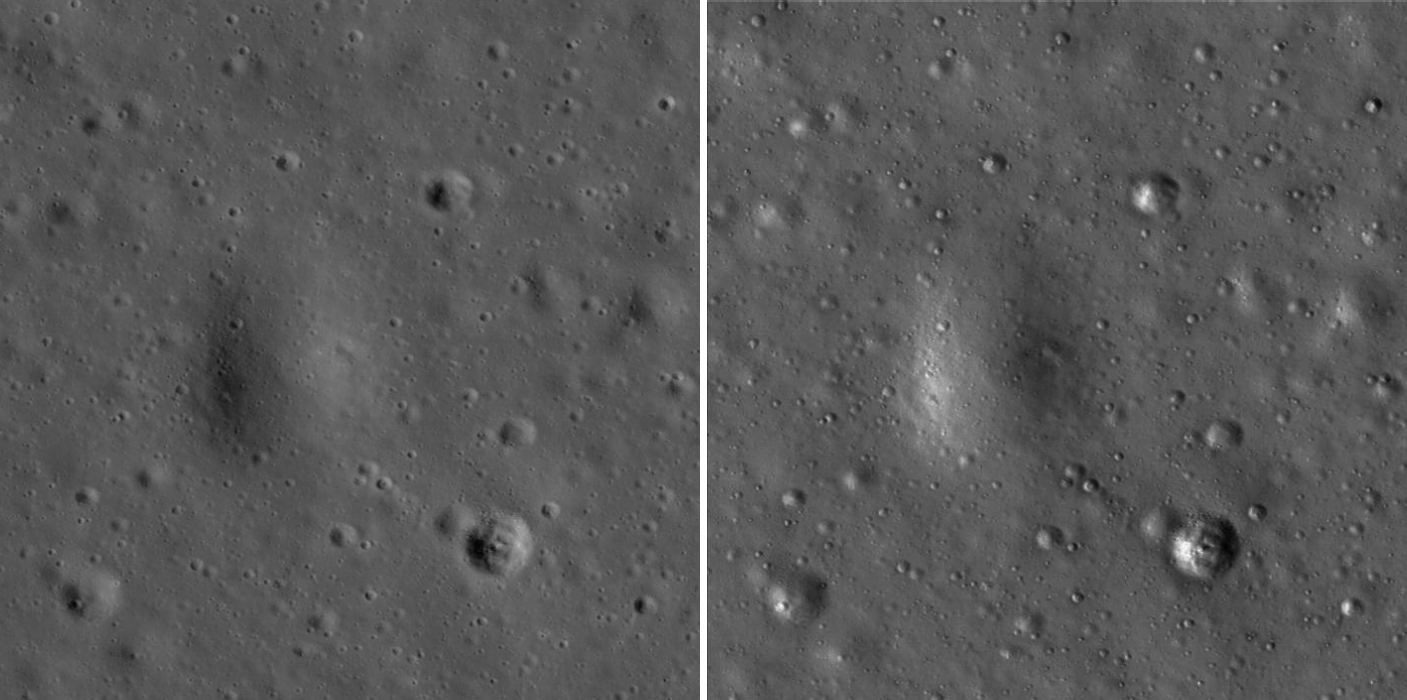
\includegraphics[width=\textwidth]{figs/craters}
	% \caption{Picture of the Apollo 15 landing site during different times of the day. The landscape is identical, but appears to be speckled with craters (lift) or hills (right). Knowing that the sun is illuminating the scene from the left and right, respectively, does explain this effect. Image credit: NASA/GSFC/Arizona State University.
	\caption{阿波罗15登陆站点在一天的不同时间的图片。景观是相同的,但是似乎是与火山口(电梯)或丘陵(右)有斑点。知道太阳从左到右分别照亮场景,确实解释了这种影响。图片来源:美国航空航天局/GSFC/亚利桑那州立大学。
	\label{fig:craters}}
\end{figure}

% More surprisingly, conceptual knowledge is often sufficient to make up for the lack of low-level cues in an image. An example is shown in Figure \ref{fig:dalmatian}. Here, a Dalmatian dog can be clearly recognized despite absence of cues for its outline, simply by extrapolating its appearance and pose from conceptual knowledge. 

% These examples illustrate both the advantages and drawbacks of a signal processing approach. While an algorithm will detect interesting signals even there where we don't see, or don't expect them (due to conceptional bias), image understanding not only requires low-level processing, but intelligent combination of the low-level cue's spatial relationship and conceptual knowledge about the world. 

更令人惊讶的是,概念知识通常足以弥补图像中缺乏低级线索。一个例子如图\ref{fig:dalmatian}所示。在这里,达尔马提亚狗可以被清楚地识别,尽管它的轮廓没有提示,只是简单地从概念知识中推断出它的外观和姿势。

这些例子说明了信号处理方法的优点和缺点。虽然一个算法会检测到有趣的信号,即使在那里我们看不到,或者不期望它们(由于概念偏差),图像理解不仅需要低级处理,而且智能组合低级提示的空间关系和关于世界的概念知识。

\begin{figure}
	\centering
		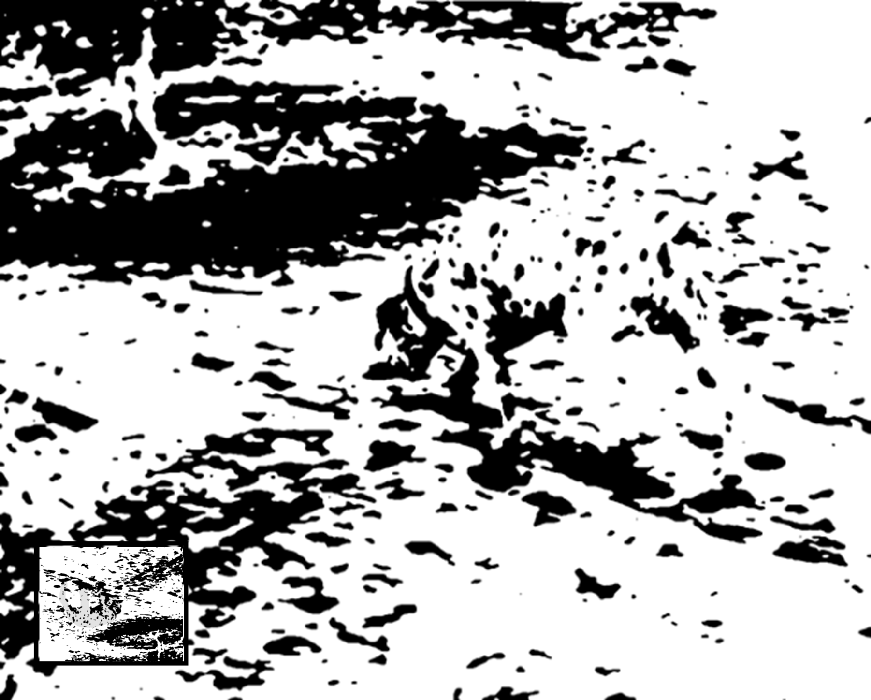
\includegraphics[width=\textwidth]{figs/dalmatian}
	% \caption{The image of a Dalmatian dog can be clearly recognized by most spectators even though low-level cues such as edges are only present for ears, chin and parts of the legs. The contours of the animals are highlighted in a flipped version of the image in the inset.
	\caption{达尔马提亚狗的形象可以被大多数观众清楚地识别,即使低级线索如边缘仅存在于耳朵,下巴和部分腿部。动物的轮廓在插图中的图像的翻转版本中突出显示。
	\label{fig:dalmatian}}
\end{figure}

% \section{Basic image operations}
% Basic image operations can be thought of as a filter that operates in the frequency or in the space (color) domain. Although most filters directly operate in the color domain, knowing how they affect the frequency domain is helpful in understanding the filter's function. For example, a filter that is supposed to highlight edges, such as shown in Figure \ref{fig:iss_edges} should suppress low frequencies, i.e., areas in which the color values do not change much, and amplify high-frequency information, i.e., areas in which the color values change quickly. The goal of this section is to provide a basic understanding of how basic image processing operation works. The methods presented here, while still valid, have been superseded by more sophisticated implementations that are widely available as software packages or within desktop graphic software.

\section{基本图像操作}
基本图像操作可以被认为是在频率或空间(颜色)域中操作的滤波器。虽然大多数滤镜直接在色域中运行,但知道它们如何影响频域有助于了解滤波器的功能。例如,假设突出显示边缘的滤波器,如图所示\ref{fig:iss_edges}应该抑制低频,即颜色值不会变化很大的区域,并放大高频信息,即,颜色值快速变化的区域。本节的目标是提供对基本图像处理操作的基本了解。这里提供的方法虽然仍然有效,但已被更多复杂的实现所取代,这些实现可广泛用作软件包或桌面图形软件。


% \subsection{Convolution-based filters}
%  A filter can be implemented using the \emph{convolution}\index{Convolution} operator that convolves function $f()$ with function $g()$. 

\subsection{基于卷积滤波器}
 可以使用函数$g()$卷积函数$f()$的\emph{convolution}\index{Convolution}运算符来实现一个过滤器。

\begin{equation}
f(x)\star g(x)=\int_{-\infty}^{\infty}f(\tau)g(x-\tau)d\tau
\end{equation}

% We then call function $g()$ a \emph{filter}\index{Filter}. As will become more clear further below, the convolution literally shifts the function $g()$ across the function $f()$ while multiplying the two. As images are discrete signals, the convolution is usually discrete

然后我们调用函数$g()$\emph{filter}\index{Filter}。如下面将会变得更加清晰,卷积逐渐地在函数$f()$上移动函数$g()$,同时使两者相乘。由于图像是离散信号,卷积通常是离散的

\begin{equation}
f[x]\star g[x]=\sum_{i=-\infty}^{\infty}f[i]g[x-i]
\end{equation} 

% For 2D signals, like images, the convolution is also two-dimensional:

对于2D信号,如图像,卷积也是二维的:
\begin{equation}\label{eq:2dconv1}
f[x,y]\star g[x,y]=\sum_{i=-\infty}^{\infty}\sum_{j=-\infty}^{\infty}f[i,j]g[x-i,y-j]
\end{equation}

% Although we have defined the convolution from negative infinity to infinity, both images and filters are usually finite. Images are constrained by their resolution, and filters are usually much smaller than the images themselves. Also, the convolution is commutative, therefore (\ref{eq:2dconv1}) is equivalent to 

虽然我们将卷积从负无穷大定义为无穷大,但是图像和滤镜通常是有限的。图像受到其分辨率的约束,并且滤镜通常比图像本身小得多。此外,卷积是可交换的,因此(\ref{eq:2dconv1})等价于

\begin{equation}\label{eq:2dconv2}
f[x,y]\star g[x,y]=\sum_{i=-\infty}^{\infty}\sum_{j=-\infty}^{\infty}f[x-i,y-j]g[i,j].
\end{equation}

% \subsubsection{Gaussian smoothing}
% A very important filter is the Gaussian filter.\index{Gaussian filter} It is shaped like the Gaussian bell function and can be easily stored in a 2D matrix. Implementing a Gaussian filter is surprisingly simple, e.g., such as

\subsubsection{高斯平滑}
一个非常重要的滤波器是高斯滤波器。\index{高斯滤波器}它的形状像高斯贝尔函数,可以容易地存储在2D矩阵中。实现高斯滤波器是非常简单的,例如,例如


\begin{equation}
g(x,y)=\frac{1}{10}
\left(
\begin{array}{ccc}
1 & 1 & 1\\
1 & 2 & 1\\
1 & 1 & 1\\
\end{array}
\right)
\end{equation}

% Using this filter in Equation \ref{eq:2dconv2} on an infinitely large image $f()$ leads to

在方程\ref{eq:2dconv2}中使用这个过滤器在无限大的图像$f()$导致

\begin{equation}\label{eq:2dconv3}
f[x,y]\star g[x,y]=\sum_{i=-1}^{1}\sum_{j=-1}^{1}f[x-i,y-j]g[i,j]
\end{equation}
(assuming $g(0,0)$ addresses the center of the matrix). What now happens is that each pixel $f(x,y)$ becomes the average of that of its neighbors, with its previous value weighted twice (as $g(0,0)=0.2$) that of their neighbors. More concretely,
\begin{equation}
\tiny
f(x,y)=
\begin{array}{lll}
f(x+1,y+1)g(-1,-1) &+f(x+1,y)g(-1,0) &+f(x+1,y-1)g(-1,1)\\
+f(x,y+1)g(0,-1) &+f(x,y)g(0,0) &+f(x,y-1)g(0,1)\\
+f(x-1,y+1)g(1,-1) &+f(x-1,y)g(1,0) &+f(x-1,y-1)g(1,1)
\end{array}
\end{equation}

% Doing this for all $x$ and all $y$ literally corresponds to sliding the filter $g()$ along the image. 

对于所有$ x $和所有$ y $,这样做对应于沿图像滑动过滤器$ g()$。

\begin{figure}
	\centering
		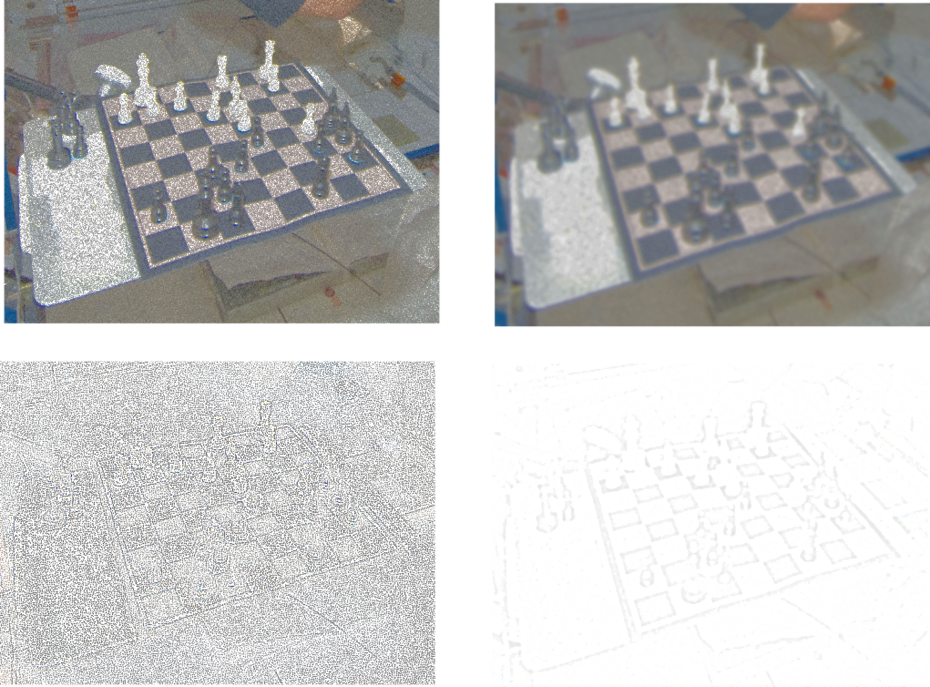
\includegraphics[width=\textwidth]{figs/filters}
	% \caption{A noisy image before (top left) and after filtering with a Gaussian kernel (top right). Corresponding edge images are shown underneath. 
	\caption{(左上)和高斯内核(右上)过滤后的嘈杂图像。相应的边缘图像显示在下面。 
	\label{fig:filters}}
\end{figure}

% An example of filter $g(x,y)$ in action is shown in Figure \ref{fig:filters}. The filter acts as a \emph{low-pass filter}\index{Low-pass filter}, suppressing high frequency components. Indeed, noise in the image is suppressed, leading also to a smoother edge image, which is shown underneath.

过滤器$g(x,y)$的一个示例在图\ref{fig:filters}中显示。滤波器作为\emph{low-passfilter}\index{低通滤波器},抑制高频分量。实际上,图像中的噪声被抑制,也导致了更平滑的边缘图像,其在下面示出。


% \subsubsection{Edge detection}\label{sec:sobel}
% Edge detection can be achieved using another convolution-based filter, the \emph{Sobel} kernel\index{Sobel filter}

\subsubsection{边缘检测}
\label{sec:sobel}
边缘检测可以使用另一个基于卷积的滤波器,\emph{Sobel}核\index{Sobelfilter}

\begin{equation}
s_x(x,y)=
\left(
\begin{array}{ccc}
-1 & 0 & 1\\
-2 & 0 & 2\\
-1 & 0 & 1\\
\end{array}
\right)
\qquad
s_y(x,y)=
\left(
\begin{array}{ccc}
1 & 2 & 1\\
0 & 0 & 0\\
-1 & -2 & -1\\
\end{array}
\right)
\end{equation}

% Here, $s_x(x,y)$ can be used to detect vertical edges, whereas $s_y(x,y)$ highlights horizontal edges. Edge detectors, such as the \emph{Canny} edge detector\index{Canny edge detector}  therefore run at least two of such filters over an image to detect both horizontal and vertical edges.

这里,$s_x(x,y)$可用于检测垂直边,而$s_y(x,y)$则突出显示水平边。因此,边缘检测器,例如\emph{Canny}边缘检测器\index{Canny边缘检测器}因此在图像上运行至少两个这样的滤波器以检测水平和垂直边缘。


% \subsubsection{Difference of Gaussians}
% An alternative method for detecting edges is the \emph{Difference of Gaussians} (DoG) method\index{Difference of Gaussians (DoG)}. The idea is to subtract two images that have each been filtered using a Gaussian kernel with different width. Both filters supress high-frequency information and their difference therefore leads to a \emph{band-pass} filtered signal\index{Band-pass filter}, from which both low and high frequencies have been removed. As such, a DoG filter acts as a capable edge detection algorithm. Here, one kernel is usually four to five times wider than the other, therefore acting as a much stronger filter.

% Differences of Gaussians can also be used to approximate the \emph{Laplacian of Gaussian}\index{Laplacian of Gaussian}, i.e., the sum of the second derivatives of a Gaussian kernel. Here, one kernel is roughly 1.6 times wider than the other. The band-pass characteristic of DoG and LoGs are important as they highlight high-frequency information such as edges, yet suppress high-frequency noise in the image.

\subsubsection{高斯差异}
检测边缘的另一种方法是\emph{差分高斯法(DoG)}\index{差分高斯法(DoG)}。这个想法是减去使用不同宽度的高斯内核过滤的两个图像。两个滤波器都抑制高频信息,因此它们的差异导致了一个\emph{带通(band-pass)}滤波的信号\index{带通滤波器(Band-pass filter)},低频和高频均已从中消除。因此,DoG过滤器用作能力边缘检测算法。在这里,一个内核通常比另一个内核宽四到五倍,因此作为一个更强大的过滤器。

高斯差分也可以用来近似高斯的拉普拉斯算子,即高斯内核的二阶导数的和。在这里,一个内核比其他内核大约是1.6倍。DoG和LoG的带通特性是重要的,因为它们突出了诸如边缘的高频信息,同时抑制了图像中的高频噪声。


% \subsection{Threshold-based operations}
% In order to find objects with a certain color or edge intensity, tresholding an image will lead to a binary image that contains ``true-false'' regions that fit the desired criteria. Thresholds make use of operators like $>,<,\leq,\geq$ and combinations thereof. There also exist adaptive versions that would adapt the thresholds locally, e.g., to make up for changing lighting conditions.

% Albeit thresholding is deceptively simple, finding correct threshold values is a hard problem. In particular, actual pixel values change drastically with changing lighting conditions and there is no such thing as ``red'' or ``green'' when inspecting the actual values under different conditions. 

\subsection{基于阈值的操作}
为了找到具有一定颜色或边缘强度的对象,对图像进行阈值化将导致包含符合所需标准的“真假”区域的二进制图像。阈值使用诸如$>,<,\leq,\geq$和它们的组合的运算符。还存在将本地适应阈值的自适应版本,例如以补偿改变的照明条件。

尽管阈值看起来很简单,但找到正确的阈值是一个难题。特别地,实际的像素值随着照明条件的改变而急剧变化,在不同条件下检查实际值时,没有像“红色”或“绿色”这样的东西。


% \subsection{Morphological Operations}
% Another class of filters are morphological operators which consists of a kernel describing the structure of the operation (this can be as simple as an identity matrix) and a rule on how to change a pixel value based on the values in the neighborhood defined by the kernel.

% Important morphological operators are \emph{erosion} and \emph{dilation}\index{Erosion}\index{Dilation}. The erosion operator assigns a pixel value with the minimum value that it can find in the neighborhood defined by the kernel. The dilation operator assigns a pixel value with the maximum value it can find in the neighborhood defined by the kernel. This is useful, e.g., to fill holes in a line or remove noise. A dilation followed by an erosion is known as a ``Closing'' and an erosion followed by a dilation as an ``Opening''. Subtracting erosed and dilated images from each other can also serve as an edge detector. Examples of such operators are shown in Figure \ref{fig:morphology}.

\subsection{形态操作}
另一类过滤器是形态运算符,其由描述操作结构的内核(这可以像单一矩阵一样简单)和关于如何基于由内核定义的邻域中的值来改变像素值的规则。

重要的形态运算符是\emph{erosion}和\emph{dilation}\index{Erosion}\index{Dilation}。侵蚀算子赋予一个像素值,该像素值具有可以在由内核定义的邻域中找到的最小值。扩展运算符分配一个像素值,该值具有在内核定义的邻域中可以找到的最大值。这是有用的,例如,填充线中的孔或消除噪声。随之而来的一次扩张被称为“封闭式”,随之而来的就是“开放”的扩张。从图像中减去图像的相减也可以作为边缘检测器。这些操作符的示例如图\ref{fig:morphology}所示。


\begin{figure}
	\centering
		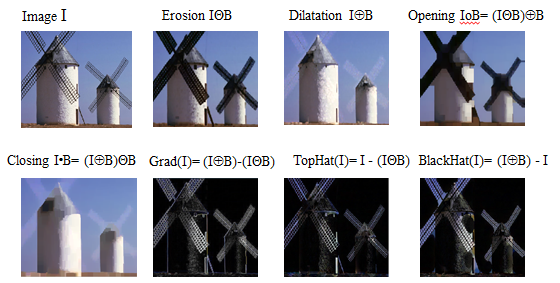
\includegraphics[width=\textwidth]{figs/morphology}
	% \caption{Examples of morphological operators erosion and dilation and combinations thereof.
	\caption{形态运算符侵蚀和扩张及其组合的例子。
	\label{fig:morphology}}
\end{figure}


% \section*{Exercises}\small
\section*{习题}\small
\begin{enumerate}
% \item Below are shown multiple ``Kernels'' that can be used for convolution-based image filtering. 

\item 下面显示了可用于基于卷积的图像过滤的多个“核”。
\item  
\begin{equation}
\nonumber
\begin{array}{|c|c|c|}
\hline
1 & 1 & 1\\
\hline
1 & 2 & 1\\
\hline
1 & 1 & 1\\
\hline
\end{array}
\quad
\begin{array}{|c|c|c|}
\hline
0 & -1 & 0\\
\hline
0 & -1 & 0\\
\hline
0 & -1 & 0\\
\hline
\end{array}
\quad
\begin{array}{|c|c|c|}
\hline
1 & 1 & 1\\
\hline
1 & -4 & 1\\
\hline
1 & 1 & 1\\
\hline
\end{array}
\end{equation}

\begin{enumerate}
% \item Identify the Kernel, which can blur an image.
% \item What kind of features can be detected by the other two kernels?

\item 标识内核,可以模糊图像。
\item 其他两个内核可以检测哪些特性?
\end{enumerate}
% \item How many for-loops are needed to implement a 2D convolution? Explain your reasoning.  

\item 需要多少个for循环来实现2D卷积?解释你的推理。
\end{enumerate} \normalsize